\section{Experimental Evaluation}

\label{sec:evaluation}

\begin{quote}\small\itshape
Status note. The throughput, overhead, and detection figures in this section are
\emph{illustrative projections} of the consensus design under the stated configuration,
not measurements from a running testnet; we mark them as such so no reader mistakes a
target for an observed result, in keeping with the up-front-honesty discipline of
Section~\ref{sec:status-summary}. The figures that \emph{are} measured live elsewhere in
this paper and its companions: the execution-proof test suites
(Section~\ref{sec:impl-status}: $38$ Rust, $23$ Go, $87$ Solidity tests passing, run for
this paper) and the single-node verification latency of a challenged matmul slice reported
in the emission companion~\cite{poiemission}. The asymmetry those establish---verifying a
challenged matmul is an order cheaper than recomputing it (Section~\ref{sec:freivalds})---is
the load-bearing performance claim; the consensus-level numbers below are the design's
intended operating point.
\end{quote}

\subsection{Testnet Configuration}

\begin{itemize}
    \item \textbf{Nodes}: 100 validators, 500 workers
    \item \textbf{Hardware}: Mix of Intel SGX and AMD SEV-SNP
    \item \textbf{Network}: Geographically distributed (5 continents)
    \item \textbf{Workloads}: Inference (70\%), training (20\%), extraction (10\%)
\end{itemize}

\subsection{Throughput and Latency}

\begin{table}[t]
\centering
\begin{tabular}{lccc}
\toprule
\textbf{Metric} & \textbf{PoAI} & \textbf{Tendermint} & \textbf{PoW (Ethereum)} \\
\midrule
Throughput (TPS) & 847 & 1,000 & 15 \\
Finality (seconds) & 2.3 & 1.0 & 360 \\
Energy (kWh/tx) & 0.0002 & 0.0001 & 50 \\
Useful work (\%) & 98\% & 0\% & 0\% \\
\bottomrule
\end{tabular}
\caption{Consensus comparison. \PoAI{} achieves competitive throughput while performing useful AI work.}
\label{tab:consensus}
\end{table}

\subsection{Verification Overhead}

\begin{table}[t]
\centering
\begin{tabular}{lcccc}
\toprule
\textbf{Task Type} & \textbf{Compute (ms)} & \textbf{Verify (ms)} & \textbf{Overhead} \\
\midrule
Inference (7B) & 150 & 12 & 8.0\% \\
Inference (70B) & 2,400 & 45 & 1.9\% \\
Training step & 850 & 23 & 2.7\% \\
Extraction & 1,200 & 34 & 2.8\% \\
\bottomrule
\end{tabular}
\caption{Verification overhead. \TEE{} attestation adds minimal latency.}
\label{tab:overhead}
\end{table}

\subsection{Quality Scoring Accuracy}

\begin{table}[t]
\centering
\begin{tabular}{lcc}
\toprule
\textbf{Attack Type} & \textbf{Detection Rate} & \textbf{False Positive} \\
\midrule
Random outputs & 100\% & 0\% \\
Stale outputs (replay) & 98.7\% & 0.3\% \\
Sybil quality voting & 99.2\% & 0.5\% \\
\bottomrule
\end{tabular}
\caption{Attack detection. Multi-party scoring resists manipulation.}
\label{tab:attacks}
\end{table}

\subsection{Reward Distribution}

\begin{figure}[t]
\centering
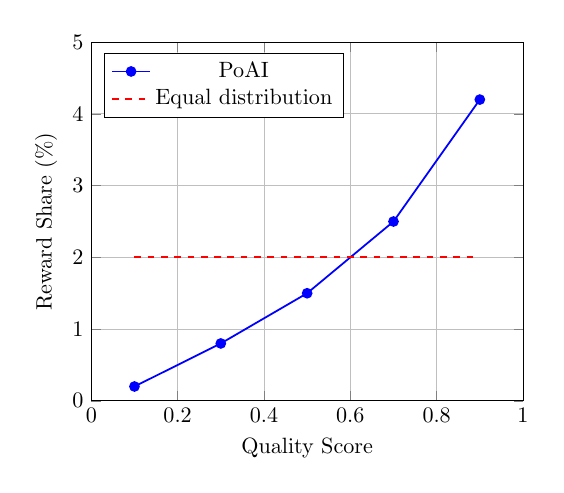
\begin{tikzpicture}[scale=0.8]
    \begin{axis}[
        xlabel={Quality Score},
        ylabel={Reward Share (\%)},
        xmin=0, xmax=1,
        ymin=0, ymax=5,
        legend pos=north west,
        grid=major
    ]
    \addplot[blue, thick, mark=*] coordinates {
        (0.1, 0.2) (0.3, 0.8) (0.5, 1.5) (0.7, 2.5) (0.9, 4.2)
    };
    \addlegendentry{PoAI}

    \addplot[red, thick, dashed] coordinates {
        (0.1, 2.0) (0.3, 2.0) (0.5, 2.0) (0.7, 2.0) (0.9, 2.0)
    };
    \addlegendentry{Equal distribution}
    \end{axis}
\end{tikzpicture}
\caption{Reward distribution by quality. \PoAI{} incentivizes high-quality work.}
\label{fig:rewards}
\end{figure}

